\begin{figure}[t]
\centering
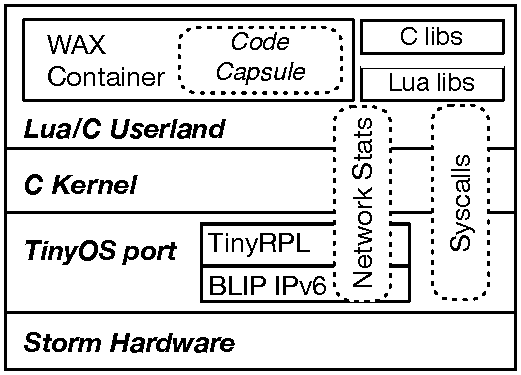
\includegraphics[width=.9\linewidth]{figs/NodeStack}
\caption{The full hardware/software stack for network experimentation. Kernel syscalls take advantage of the synergy between hardware and firmware to expose low-level metrics on the radio stack that would otherwise be difficult to incorporate.}
\label{fig:nodestack}
\end{figure}

\section{Evaluation Platform}



Traditionally, the storage constraints of embedded platforms have forced an opacity onto embedded networking stacks, making it difficult to add monitoring logic without removing functionality from the stack itself.
The iterative process of altering the networking stack for any sort of parametric study is intractable for more than a few parameters.
Usually, these parameter spaces are explored with the help of a network simulator such as COOJA~\cite{cooja}, OMNET++~\cite{omnet++} or NS2~\cite{ns2}.
While helpful for establishing estimates of how a protocol under a set of parameters might perform, it is difficult to evaluate the practicality of a protocol without having implemented it in a real system.

Using a modern platform with relaxed storage constraints and increased programmability, we demonstrate a novel platform for full-stack network monitoring on real-world WSN deployments.
To facilitate empirical studies, we construct a mechanism that enables chunks of Lua code to be disseminated over a network, safely assembled on each node, and then executed to subject the full network to a well-defined load or traffic pattern.
These \emph{code capsules} define the start and end conditions of an experiment, pattern generation, data acquisition and report delivery.

\subsection{Hardware Platform}

The hardware platform for typically used network evaluations is the TelosB mote (used in \cite{ko2011evaluating} and modeled in COOJA for network simulations).
The TelosB, introduced in 2005~\cite{polastre2005telos},  employs a 16-bit MSP430 microprocessor with 48 KB ROM and 10 KB RAM.
This was ample space 10 years ago, but as the size and complexity of IPv6 standards and routing standards increased, the increased pressure on code space informed a set of compromises in the design of the TinyOS networking stack, our focal operating system.
These compromises and how they affect the our goal of iterative, parameter-driven evaluation are explored in more detail below.

The recently-introduced Storm platform~\cite{andersen2016system} used in this study has a 32-bit ARM Cortex M4, with 512 KB ROM and 64 KB RAM, offering much more processing power and storage capabilities.


\subsection{Software Platform}


In this section, we discuss the software platform for the Storm motes that are the nodes used in the networking study presented in Section~\ref{section:evaluation}.
The motes run a port of TinyOS 2.x, using the Berkeley Low-Power IPv6 stack (BLIP) and TinyRPL.
Over this, the nodes run the Synergy kernel with a Lua userland~\cite{andersen2016system}, which introduces a dynamic, scripting environment with visibility into the inner workings of the operating system (and thus network stack).
We extend this base functionality with:
\begin{itemize}
\item a set of new syscalls with the ability to edit routing and neighbor tables, and view control traffic and other network telemetry,
\item a network measurement platform Lua library for conducting networking studies
\item a host of tricks for placing two complete routing protocols on a mote with the ability to switch without reflashing
\end{itemize}

Figure~\ref{fig:nodestack} illustrates the full mote platform that runs on each node in the network to be measured.
When each node boots, it first performs the usual TinyOS initializations, and then jumps into the userland code and starts executing the equivalent of \texttt{main.lua}.
We preempt this boot sequence so that before the userland code is executed, the kernel reads from a particular location in external memory that establishes which routing protocol and parameters it should use.
This requires some trickery, described below.
Once in \texttt{main.lua}, the network measurement platform performs its initialization before jumping into the received code capsule to start the experiment.

Each experiment is started and coordinated by either a laptop or desktop computer attached to the network.
This coordinator disseminates code, triggers the beginning of the experiment and retrieves the reports from the nodes after the experiment.
The coordinator does not participate in the experiment, but it can serve as a ``data drop'' for for measurement application such as for measuring the packet reception ratio.

\subsection{Synergy Kernel and Lua Userland}

\begin{table*}[ht]
\centering
\begin{tabular}{| l | l |}
\hline
\textbf{Syscall} & \textbf{Description} \\ \hline \hline
\multicolumn{2}{|c|}{\texttt{StormSysInfoP.nc}} \\ \hline
\verb`storm.net.retrystats()` & Retrieves transmission and retransmission counts \\ \hline
\verb`storm.net.thopstats()` & Retrieves number of RS and RA with 3hop options sent \\ \hline
\verb`storm.net.rplstats()` & Retrieves number of DIO, DIS and DAO messages sent \\ \hline
\verb`storm.net.stats()` & BLIP-stats: packets sent, forwarded, dropped, fragmented \\ \hline
\multicolumn{2}{|c|}{\texttt{StormRoutingTableP.nc}} \\ \hline
\verb`storm.os.addroute(pfx, len, nhop, iface)` & Add route via nexthop over given interface to routing table \\ \hline
\verb`storm.os.delroute(routekey)` & Removes given route from routing table \\ \hline
\verb`storm.os.lookuproute(pfx, pfx)` & Returns routing table entry matching the given prefix, length \\ \hline
\verb`storm.os.gettable()` & Returns all valid entries in the routing table \\ \hline
\verb`storm.os.flushroutes()` & Deletes all entries from the routing table \\ \hline
\verb`storm.os.flushneighbors()` & Deletes all entries from neighbor table \\ \hline

\end{tabular}
\caption{List of new syscalls implemented for stack monitoring. Each of the \texttt{stats()} methods has a corresponding \texttt{clear()} to erase the cumulative counts.}
\label{table:syscalls}
\end{table*}

A detailed study of a layer 3 routing protocol, such as RPL, needs to be able to pull information from layer 2 and layer 1 components in the networking stack.
The Synergy kernel exposes TinyOS functionality to userland applications through the use of syscalls, giving applications the ability to run timers, send or receive network traffic, and write to GPIO pins or other peripherals.
These syscalls are supported within TinyOS by a set of drivers, which are special TinyOS components.
We add two additional drivers: \texttt{StormRoutingTableP.nc}, which lets applications view and edit the routing and neighbor tables in BLIP; and \texttt{StormSysInfoP.nc}, which exposes routing state, packet counts, retry counts and routing control traffic counts, among other statistics.
A list of the added syscalls can be found in Table~\ref{table:syscalls}.

(Embedded) Lua~\cite{elua} is an embeddable, lightweight, stack-based, high-level scripting language that is easily extensible in C.
Because Lua is an interpreted language, we can add new code at runtime in the form of \emph{code capsules} which we disseminate through a network.
Deployed applications can get large (1800 bytes for a simple traffic generation program) compared to 802.15.4 frames, which are only 127 bytes, predicating the need for a code reassembly mechanism.
The mechanism for dynamically adding logic to a running mote is enabled through a C function that accepts string buffers that contain segments of code.
We deliver code over TCP, using a recent adaptation of the BSD TCP stack to TinyOS.
Each mote listens on a known port for incoming code segments, and hands them to the built-in Lua-C API function \texttt{LuaL\_loadbuffer}, which attempts to evaluate the buffer as a chunk of Lua code.
If the chunk is ``complete'' --- that is, a syntactically valid piece of Lua code --- then it is executed, the results are placed on the Lua stack and interpreted, and the buffer is emptied.
Out-of-memory errors can occur if a buffer forms a large Lua code segment that is not terminated (such as within a large \texttt{while} statement).
It is difficult to recover from out-of-memory errors on an embedded platform; this encourages the dissemination of small, modular functions or tuning variables for preloaded applications.

%\todo{talk about how we can replace methods at runtime. Can have a generic method that calls the 'pattern generator' every 'N' seconds, and we can replace those params and functions to do whatever we want. Provide a code sample!}

\subsection{Network Measurement Platform}

Each network experiment comprises five elements: initialization, start condition, traffic generation, stop condition, reporting.
Our network measurement platform provides default methods for each of these elements, and new methods and data structures can also be disseminated over the network and used in subsequent experiments.
Code capsules sent over the network and received at each node describe the state machine of actions to be taken over the course of a network experiment.

\begin{figure*}[ht]
\centering
\includegraphics[width=.9\linewidth]{figs/code_dissemination}
\caption{Code dissemination over WSN nodes. Each node contains the stack in Figure \ref{fig:nodestack}. Code is disseminated from a coordinator node via unicast to each node. After the experiment is complete, reports are sent back to the coordinator.}
\label{fig:dissemination}
\end{figure*}

Now, we will describe how the platform implements each of these five elements.

\textbf{Initialization}: The initialization of a code capsule occurs when the kernel first jumps into the userland memory and begins executing.
The initialization sets up vital resources and methods for the network measurement platform.
It opens sockets to receive code capsules and commands for execution, and allocates memory and initializes the internal log for telemetry storage.
Depending on how the network experiment is run, the initialization of a node may also erase its neighbor and routing tables to return the node to a ``just booted'' state, but without the typical loss of dynamically loaded code stored in RAM.
This is also the time when any code would be loaded from the external flash memory and executed.

\textbf{Start}: Each network experiment can define its own trigger.
For complex network measurements, this may be accomplished with the aid of a time synchronization technique, but in the small networks we are currently investigating, a simple ``flood-sleep-reset-start'' method suffices.
This method can actually be disseminated through the network, allowing the start method to be customized for the experiment at hand.

The code for the flooding start mechanism used for our network measurements is below.
It defines a socket with a callback invoked when the socket receives a packet.
The callback schedules a software reset\footnote{This can be switched out for a routing/neighbor-table flush to persist dynamically loaded code} to be execued in 20 seconds (configurable), and also schedules the three ``reset'' broadcast packets to be sent with some jitter between them.
Jitter helps increase the probability that all nodes receive a reset signal; otherwise, if multiple nodes both receive a reset broadcast and they send a broadcast at the same time, those broadcasts may collide at a third node such that it does not receive either.

\begin{luacode}
-- base wait of 20 seconds
wait = 20
-- listen on port 6666 for reset commands
rsock = storm.net.udpsocket(6666, function()
 -- truncate flooding
 if not heard_reset then
  heard_reset = true
  storm.os.invokeLater(wait*SECOND, storm.os.reset)
  cord.new(function()
   for i=1,5 do
    -- jitter on bcast to avoid conflicts
    sleep(3*SECOND)
    storm.net.sendto("ff02::1", 6666 "reset!")
   end
  end)
 end
end)
\end{luacode}

Once the function has been disseminated to all nodes, we choose a node to start the flooded reset by sending the following code capsule to any node, which broadcasts the reset command on behalf of the coordinating computer which has no 802.15.4 radio.

\begin{luacode}
storm.net.sendto("ff02::1",6666,"reset!")
\end{luacode}

We could also of course send a packet to port 6666 on a node, which would then start the flooding process, but by having the original node broadcast, we can reduce the flooding time by a few seconds\footnote{It is also much more fun to execute code over the network rather than just sending a packet}.

\textbf{Traffic Generation:}  This block of code is the logic that runs during the experiment in question and handles both traffic generation and network monitoring.
The primary concerns of the generation component are determing how often the node sends and to whom.
The two most common patterns of this are a periodic send or a request-response or ``echo'' generator.
The event-driven nature of the userland networking interface facilitates these patterns of traffic generation.
For example, the logic to respond to a request can be invoked in the callback for a received packet on a given port.
Additionally, dynamic code loading allows capsules to easily define point-to-multipoint, multipoint-to-point or even point-to-point traffic.

Monitoring and statistical code for the eventual report is interspersed in the capsule logic for generating traffic and notifications of received traffic.
Beyond the network statistics provided by the kernel interface (described in Table~\ref{table:syscalls}), it is up to the code capsule to determine the logic for what statistics are kept.
The standard data structures provided by Lua (integers, tables and arrays) coupled with storage syscalls for writing to the log enable the composition of most common reporting and statistical techniques: maps/tables, histograms and counters.

By storing data in non-volatile flash memory as the experiment is run, we can maintain a separation from the execution of the study, removing a reliance on the targeted network or protocol to report the data.
Network partitions and ``black holes'' are very real possibilities in wireless sensor network research.
If telemetry data is not stored locally during an experiment and instead used as the application traffic, then any network issues (including the period at the beginning of an experiment when routing has not been established) result in a loss of data.

\textbf{Stop Condition:}
The reporting phase of an experiment is a distinct phase to avoid the act of reporting statistics interfering with the behavior of the network under study.
Each network experiment defines a ``stop'' condition, which can be defined by sending a certain number of packets, sending traffic for a certain amount of time, or receiving a ``stop'' signal from the coordinating node.
Here, it is often helpful to cancel timers or erase callbacks upon receiving the stop condition so that the network experiment does not continue to send data, adjust routing and mutate data structures while reporting is taking place.

\textbf{Reporting:}
From our new syscalls, we can retrieve the following information:
\begin{itemize}
\item The number of transmitted packets, including the number of software retransmissions
\item The number of IPv6 neighbor discovery messages sent and received (Solicitations and Advertisements)
\item The number of packets sent, forward, dropped or fragmented
\item How many DIS, DIO and DAO messages sent and received by the RPL implementation
\item The number and identities of routing and neighbor table entries
\item The current hop count or rank of the node
\item A sequence number to track the order of samples
\end{itemize}

The network experiment samples these values at regular intervals and saves them as fixed-size records in the Storm's external flash.
These logs start at a given memory position and advance upward.
During the reporting phase, the log is replayed from the start position and the node transmits collections of records to a collection point (typically the coordinator node).
As part of the stop condition for a network experiment, the network measurement platform writes a \texttt{truncate} record to the log to indicate a stopping point for log replay.

\subsection{Tricks and Limitations}

\textbf{Multiple Routing Protocols.} Traditionally, due to memory constraints, switching between routing protocol implementations has required reprogramming (``reflashing'') each individual mote, which is a lengthy and manual process that quickly becomes tedious at even modest numbers of motes.
The ample memory on the Storm platform enables the simultaneous placement of multiple routing protocol implementations on the same mote.
This becomes possible with some careful overlapping of large data structures (such as routing-protocol specific neighbor tables).
We choose to overlap data structures and not the routing code itself, because the \texttt{event}s raised by TinyOS components upon receiving packets or interrupts can only be created at compile time.

The easiest way to switch between routing protocols is at boot time: the Kernel decides which routing protocol to start by reading a particular memory location for a flag value.
While conceivably one could avoid this reboot by calling ``stop''\footnote{Using TinyOS's \texttt{StdControl} interface, which provides both \texttt{.start()} and \texttt{.stop()} methods} one routing protocol and switch to another, this would also require stopping and cancelling the family of timers and triggers required by the previously running routing protocol.

We use \texttt{\_\_attribute\_\_(section("name"))} to place data structures from different routing protocols at the same locations in memory to save space.
We do not run into conflicts as long as only a single routing protocol accesses these data structures, otherwise we risk corrupting metadata or reading invalid data.
Because we cannot protect against methods being called by TinyOS while the system is running, we augment the routing protocol implementations to abort before accessing overlapping data structures if it is not the active protocol.

\textbf{Dynamic Code Limitations.} A limitation of the current version of dynamic code loading is that the code is saved to RAM, which is lost on reboot.
This places limits on what code must be placed on the mote before deployment and what code can be dynamically loaded over the network after the mote is deployed.
Broadly, these constraints force low-level routing protocol code to be programmed into the ROM (not lost on reboot) of each mote, along with the methods handling code reassembly and the basic methods for the network measurement platform described below.
Custom telemetry methods and experiment execution scripts can be loaded dynamically over the network.

A possible solution for removing this limitation uses the external flash memory on the Storm board to store Lua program text, and then introduce a flag read on boot that performs the above process by loading code from memory rather than receiving over the network.
The disadvantage here is that the textual representation of Lua code is much larger than the resulting symbols, so this would dramatically reduce the amount of log space available for the networking management platform.

%The storage constraints of the older platforms on which BLIP and TinyRPL were developed led to the use of compile-time configuration options (e.g. \verb`#define` and \verb`#ifdef`) to remove unused features from the compiled stack when flashing motes.
%Although the Storm platform does not possess the same storage constraints, the status of the current codebase limits the ability to use userland applications to configure the TinyOS networking stack.
%Refactoring the codebase to use run-time rather than compile-time parameters is a not insignificant task, but the WAX methodology could be easily extended to pass configuration options to the TinyOS networking stack to change the choice of objective function or other RPL parameters.

\if 0
talk about tinyos? blip?

Many recent features of  ipv6 nd not implemented
many constants vital to the protocol buried deep in header files with #define so that they
  can be placed into more plentiful ROM. Can't be edited at runtime
\fi

\if 0
- many prior measurements done exclusively on simulators
    - few experiments run in the real world
    - if using a Java implementation, can totally put in all features you want and
      easy to chagne parameters, but this doesn't help us evaluate how well protocol works
- Hardware:
    - advancements in hardware make


- establish the measurement apparatus for these:
    - TinyOS Kernel
    - Syscalls in Lua
        - challenges developing syscalls
    - Dynamic code loading in Lua
    - fitting everything into the mote
        - memory issues
        -  trigger issues: receive a rogue message can mess everything up because function is still there and wired up!
    - "WAX stack"
        - follow similar structure to the sensys paper
        - the components of a network experiment code
        - how to we do logging, where it goes
\fi
